%%%%%%%%%%%%%%%%%%%%%%%%%%%%%%%%%%%%%%%%%%%%%%%%%%%%%%%%%%%%%%%%%%% 
%                                                                 %
%                            CHAPTER FOUR                          %
%                                                                 %
%%%%%%%%%%%%%%%%%%%%%%%%%%%%%%%%%%%%%%%%%%%%%%%%%%%%%%%%%%%%%%%%%%% 
 



\chapter{CONVERGENCE MODEL} \label{sec:mathmodel}
\section{Convergence Model}
Researchers have long argued that every social network has a tendency
towards balanced states~\cite{Doreian:02}. The balance aspect of ``network evolution" becomes a non-trivial problem when relationships are measured numerically. Given an initially imbalanced network, it is interesting to see what state the network will converge to. We propose a model that characterizes a social network's convergence in this chapter.

It is noted in social psychology literature that people are reluctant
to make changes in relations as they tend to avoid the effort needed to
make such changes. In a balanced triadic relation, participants are
likely to do nothing and keep their pairwise relations as what they
were. In an imbalanced triadic relation, participants are likely to
make the smallest effort possible to regain triadic balance. We define
the concept of relation cost as the effort one needs to take to
accomplish a certain relation change. Our convergence model is
established based on a unified assumption: every social network
converges in a way that requires as little total change in relations
as possible to reach a balanced state.

By definition~\ref{alternative def}, every layout in the Euclidean
space automatically satisfies the metric triangle inequality, and
hence corresponds to a balanced state of the network.  For an
imbalanced social network, it is not possible to draw it using its
initial relation distances.  Hence, our convergence model aims to
produce a layout of the social network with minimum total relation
cost from the original one.

Let $G=(V,E)$ denote an arbitrary social network, and $G^{*}=(V,
E^{*})$ denote a balanced state of $G$. Let $n*n$ matrix $X$ denote
the layout of $G^{*}$, with each row vector $x_{i}$ denoting node
$i$'s location in $m$-dimensional space. For each pair $(i,j)$,
$\psi(i,j)$ denotes its relation distance in $G$, and $d_{i,j}(X)$
denotes distance between $i$ and $j$ in $X$, i.e., its relation
distance in $G^{*}$.  Given an edge $(i,j)\in E$, we consider the
relation cost on $(i,j)$ is given by:
\[c_{i, j}(X)=w_{\psi(i,j)}*(d_{i,j}(X)-\psi{(i,j)})^2\]
where the weight value is a function of the original distance. The
weight function can take into account the difficulty of changing a
relation. For example, it is generally easier to change a neutral
relation than a positive or negative relation that carries with them
initial bias. The study of optimal weights is beyond the scope of this
thesis. However, we consider three main classes of weights:
\[
 w_{\psi(i,j)}= \left\{ 
  \begin{array}{l l}
    w_{+} & \quad \text{if $\psi(i,j)$ is a positive edge}\\
    w_{O} & \quad \text{if $\psi(i,j)$ is a neutral edge}\\
    w_{-} & \quad \text{if $\psi(i,j)$ is a negative edge}\\
  \end{array} \right.
\]

If $w_{O} << w_{+}$ and $w_{O} << w_{-}$, then neutral edges would
have very little influence on the already established
positive/negative relations.

\begin{definition}
Let $G=(V,E)$ be a social network where $E$ is a set of weighted
edges. Its converged network $G^{*}=(V,E^{*})$ is given by layout
matrix $X$ with $d_{i,j}(X)$ as the relation distance between every
pair $(i,j)$, such that the total relation cost $\sigma(X)$ is
minimized,
\[\sigma(X)= \min_{X} \sum_{i<j \leq n}w_{\psi(i,j)}*(d_{i,j}(X)-\psi{(i,j)})^2\].

\end{definition}
The optimization of relation cost is in fact a Metric
Multidimensional Scaling problem (MDS) by assigning nodes a location
in metric space. The total cost function is called stress in MDS, and
is often minimized through an optimization strategy called {\it stress
  majorization} \cite {Gansner:05}. Stress majorization is an iterative
method that guarantees monotonically decreasing stress in each
iteration, and returns a locally minimum solution.  It is recognized
as a principled technique in the field of graph drawing. The
algorithm, however, requires $O(n^3)$ time and $O(n^{2})$ space. Due
to its complexity, stress majorization is applicable on graphs with
limited size. We discuss the algorithmic problem of stress majorization in Chapter 5.

\section{Predictability of Convergence Model}\label{predictability}
A successful convergence model will help justify the balance tendency of social networks, and hence support the balance theory behind it. Moreover, convergence model inherits a predictive power as it models the dynamic nature of social networks. For example, the strong triadic closure states that two people with a common close friend are very likely to friend each other in the future~\cite{Granovetter:1973}. We have argued in Table~\ref{tab:imbalanced_extended} that triad ``$s+, s+, O$" is imbalanced, it is important to verify if such a triad will converge to ``$s+, s+, +$" accordingly in the convergence model. Some frequently seen dynamic phenomenon in social networks are listed below, which we expect a congruent convergence model will be able to explain. The concept of strong and weak ties follows what is described in Table~\ref{ref:rel_types}. Following the discussion in section~\ref{relation distance}, we partition the relation distance by the same constraints in Table~\ref{tab:constraints}. We illustrate and prove these propositions under our convergence model.

 In the demonstration examples shown in Figure~\ref{demo1}, Figure~\ref{demo2} and Figure~\ref{demo3}, the boundary parameters are chosen as the following: $b_{s+}=0.1,\, b_{w+}=0.5,\,  b_{w-}=0.7,\,b_{s-} = 1.1$. The relation distances of strongly positive relation, weakly positive relation, neutral relation, weakly negative relation, strongly negative relation are picked as 0.1, 0.3, 0.6, 0.9, 1.1 respectively. Notice that the parameters is arbitrarily picked for the purpose of demonstration. Other configurations are legitimate as long as the constraints in Table~\ref{tab:constraints} are satisfied. As it is discussed previously, we constrain $w_{0}$ such that $w_{0}<< \min{\{w_{+}, \, w_{-}\}}$. In the demonstration examples, the weights are chosen as: $w_{+}=w_{-}=1,\, w_{0}=0.001$.
 
 In the proofs below, we denote $G$ as the initial network and $\cal G$ as its balanced state after convergence. The initial distance of a neutral relation is denoted as $\delta_{0}$. Clearly, $b_{w+} \leq \delta_{0} \leq b_{w-}$ holds.
 
\begin{proposition}\label{closure}
Strong Triadic Closure Property. Let $(A,B,C)$ be a triad of interest. If both $(A,B)$ and $(B,C)$ are strongly positive relations in a social network, then $(A,C)$ will be a positive relation in the balanced state.
\end{proposition}
Illustrated in (1) of Figure~\ref{demo1}, initially edges $(0,1)$ and $(1,2)$ are given as strongly positive. In its converged layout, node $0$, node $1$ and node $2$ are on the same line with node $1$ in the middle. Hence, $d_{02}$ is twice as much as $d_{01}$ ($d_{12}$). As a result, $(0,2)$ turns to be a weakly positive edge as desired. 

{\bf Proof.} We need to prove that the initially unconnected $(A,C)$ will become a positive edge in $\cal G$. Also, we need to show $(A,B)$ and $(B,C)$ will remain strongly positive in $\cal G$. 

Initially, $\psi{(A,B)} + \psi{(B,C)} < 2b_{s+}<b_{w+}<\delta_{0} =\psi{(A,C)}$. $A$, $B$, $C$ cannot coexist in the space without change some of the distances. To reach a balanced structure, it is either going to stretch $(A,B)$ and $(B,C)$, or to shrink $(A,C)$ in space. But in either way or a combination of both, the least modification, which indicates the smallest relation cost, occurs when $A$, $B$, $C$ stays in a line with $B$ in the middle. 
Let the length of both $(A,B)$ and $(B,C)$ be $l_{1+}$ and $l_{2+}$, and the length of $(A,C)$ be $l_{0}$. The total relation cost should be the following.
\[
\sigma(l_{1+}, l_{2+} l_{0}) = \min_{l_{1+},l_{2+}, l_{0}} w_{0}(l_{0}-\delta_{0})^2 + w_{+}(l_{1+}-\psi{(A,B)})^2+ w_{+}(l_{2+}-\psi{(A,B)})^2
\]
\[
\text{subject to  } l_{0}=l_{1+}+l_{2+}.
\]
The optimization problem can be rewritten as the following,
\[
\sigma(X)= \min_{X}\, 1/2X^{\top}HX+C^{\top}X+ \alpha,
\]
where $\alpha$ is a constant and
\[
 X =
 \begin{pmatrix}
  l_{1+}  \\
  l_{2+},
 \end{pmatrix},
  H =
 \begin{pmatrix}
  2(w_{0}+w_{+}) & 2w_{0}\\
  2w_{0} & 2(w_{0}+w_{+})
 \end{pmatrix},
  C =
 \begin{pmatrix}
  -2(w_{0}\delta_{0}+w_{+}\psi(A,B))  \\
  -2(w_{0}\delta_{0}+w_{+}\psi(A,C))
 \end{pmatrix}.
\]
Let  $\frac{\mathrm d}{\mathrm d X} \big( \sigma(X) \big)=0$. We have $X=-H^{-1}C$,
\[
  X=\left\{ 
  \begin{array}{l l}
    {l_{1+}} = {{w_{0}\delta_{0}+(w_{0}+w_{+})\psi(A,B)-w_{0}\psi(B,C)} \over {2w_{0}+w_{+}}}\\
    {l_{2+}}={{w_{0}\delta_{0}+(w_{0}+w_{+})\psi(B,C)-w_{0}\psi(A,B)} \over {2w_{0}+w_{+}}}
  \end{array} \right.\text{ ,}
\]
and
\[
l_{0}=l_{1+}+l_{2+} ={{2w_{0}\delta_{0}+w_{+}(\psi(A,B)+\psi(B,C))} \over {2w_{0}+w_{+}}} \text{ .}
\]
By constraint $w_{0}<<w_{+}$, we have
\[
{l_{1+}}=\psi(A,B)+{{w_{0}(\delta_{0}-\psi(A,B)-\psi(B,C))} \over {2w_{0}+w_{+}}} \simeq \psi(A,B)
\]
Similarly, ${l_{2+}} \simeq \psi(B,C)$. Hence, both $(A,B)$ and $(B,C)$ will remain strongly positive. Now, $l_{0} \simeq \psi(A,B)+ \psi(B,C) < b_{w+}$, and therefore $(A,C)$ will become a positive relationship. $\Box$\\

\begin{figure}[th]
\centering
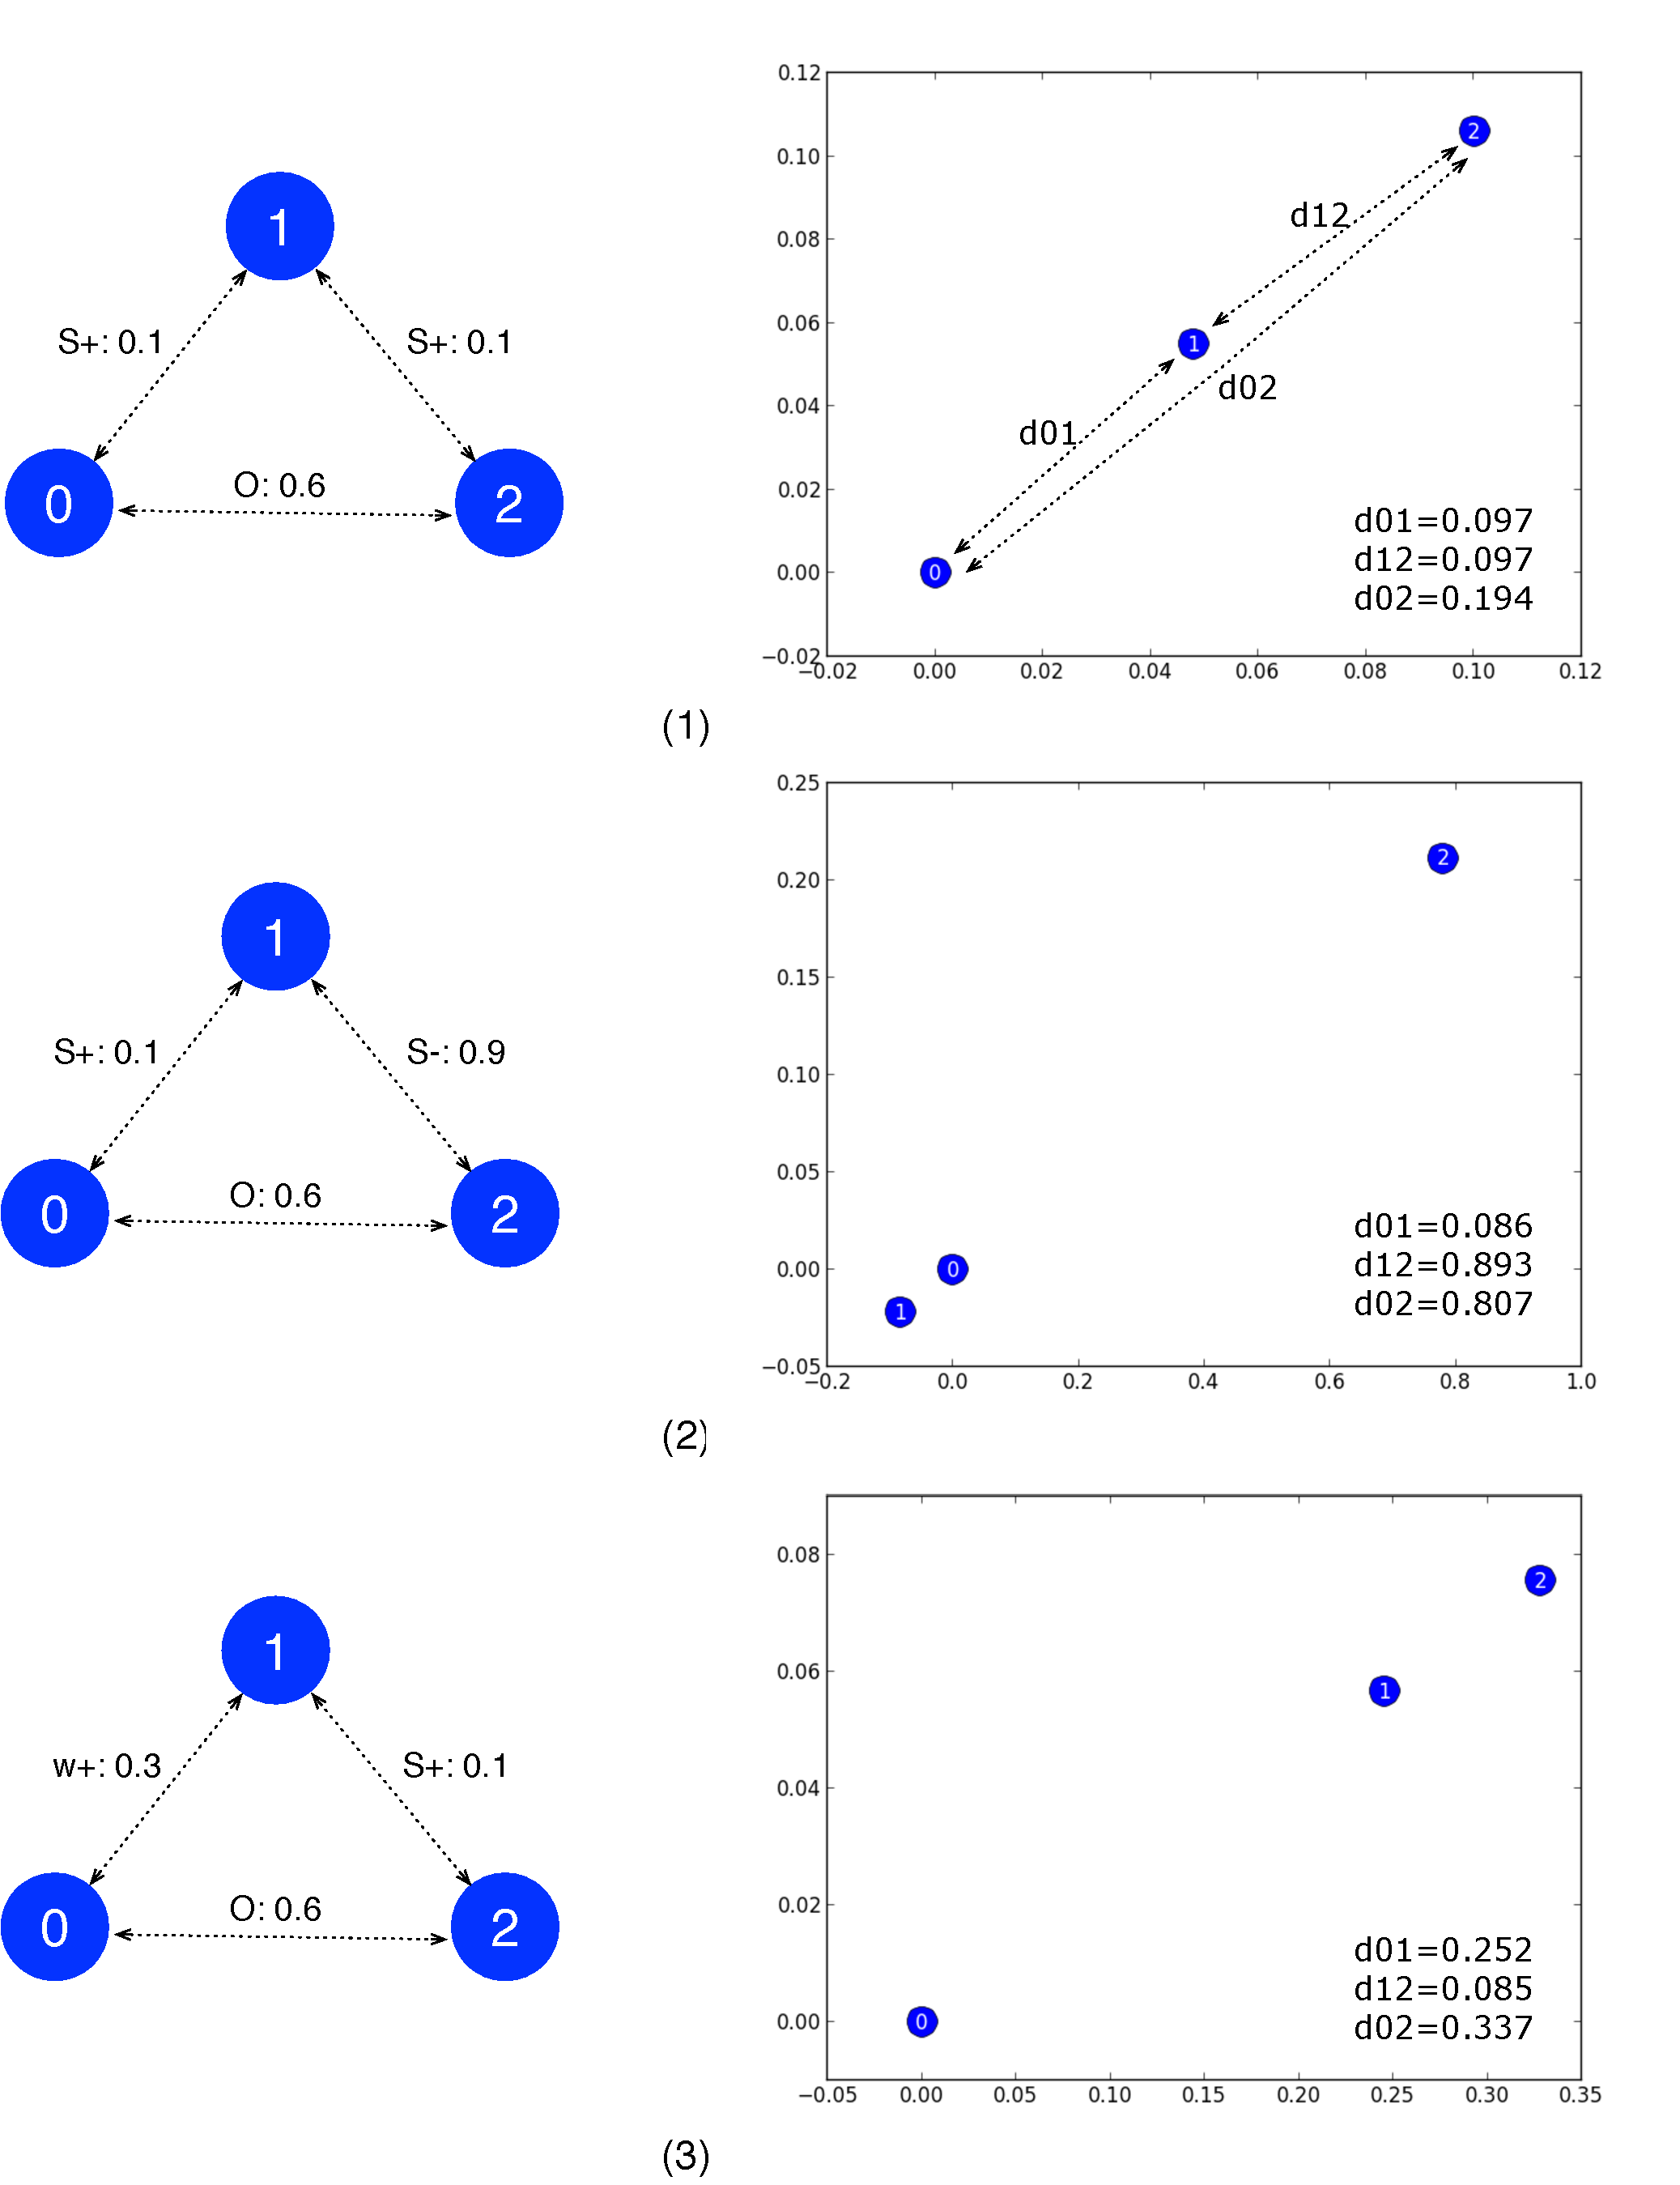
\includegraphics[height=5.5in]{Figs/demo1.pdf}
\caption{\label{demo1}The demonstration experiments of Propositions~\ref{closure}, \ref{neutralization} and \ref{attenuation}. Each blue ball has a white number $i$ in it, indicating node $i$. The initial state of each triad is shown in figures on the left, and the corresponding converged layouts on the right.}
\end{figure}
\begin{proposition}\label{neutralization}
Neutralization Property. Let $(A,B,C)$ be a triad of interest. If $(A,B)$ is strongly positive and $(B,C)$ is strongly negative, then $(A,C)$ will be negative in the balanced network, and the strength of $(A,C)$ should be no stronger than the strength of $(B,C)$.   
\end{proposition}
The first part of the neutralization property can be seen as a twin property of strong triadic closure with negative sign. It says if A has a friend B and a strong enemy C, then B and C will not get along in the long run. The second part is an inference assumption; one argument for the assumption is: ``the later established disliking is not likely to be stronger than the original hatred that causes the disliking". 

Illustrated in (2) of Figure~\ref{demo1}, initially edge $(0,1)$ is given as strongly positive while edge $(1,2)$ is given as strongly negative. In its balanced layout, node $0$, node $1$ and node $2$ are on the same line with node $0$ in the middle. Hence, $d_{02}$ equals $d_{12}-d_{01}$, which is in the range of negative relations. 

{\bf Proof.} We need to prove $(A,C)$ will become a negative edge in $\cal G$, and that $(A,C)$ will not be longer than $(B,C)$ in metric space. Also, we need to prove $(A,B)$ and $(B,C)$ will remain what they were in $\cal G$. 

By similar arguments in the proof of Proposition~\ref{closure}, $A$, $B$, $C$ cannot coexist in the space without change some of the distances. To reach a balanced structure, it is either going to stretch $(A,B)$ and $(A,C)$, or to shrink $(B,C)$ in space. But in either way or a combination of both, the least modification, which indicates the smallest total relation cost, occurs when $A$, $B$, $C$ stays in a line with $A$ in the middle. Let the length of $(A,B)$ be $l_{+}$, the length of $(B,C)$ be $l_{-}$ and the length of $(A,C)$ be $l_{0}$. The total relation cost on ($A$, $B$, $C$) during the convergence should be the following.
\[
\sigma(l_{+}, l_{0}, l_{-}) = \min_{l_{+}, l_{0}, l_{-}} w_{0}(l_{0}-\delta_{0})^2 + w_{+}(l_{+}-\psi(A,B))^2+w_{-}(l_{-}-\psi(B,C))^2
\]
\[
subject\,\,to  \quad l_{0}+l_{+}=l_{-}.
\]
The optimization problem can be rewritten as the following,
\[
\sigma(X)= \min_{X}\, 1/2X^{\top}HX+C^{\top}X+ \alpha,
\]
where $\alpha$ is a constant and
\[
 X =
 \begin{pmatrix}
  l_{0}  \\
  l_{+},
 \end{pmatrix},
  H =
 \begin{pmatrix}
  2(w_{0}+w_{-}) & 2w_{-}\\
  2w_{-} & w(w_{+}+w_{-})
 \end{pmatrix},
  C =
 \begin{pmatrix}
  -2(w_{0}\delta_{0}+\psi(A,C))  \\
  -2(w_{+}\psi(A,B)+\psi(B,C))
 \end{pmatrix}\text{ .}
\]
Let  $\frac{\mathrm d}{\mathrm d X} \big( \sigma(X) \big)=0$. We have $X=-H^{-1}C$, 
\[
  X=\left\{ 
  \begin{array}{l l}
    {l_{0}} = {{(w_{+}w_{0}+w_{0}w_{-})\delta_{0}+w_{+}\psi(A,C)-w_{+}w_{-}\psi(A,B)} \over {w_{0}w_{+}+w_{+}w_{-}+w_{0}w_{-}}}\\
    {l_{+}}={{(w_{+}w_{0}+w_{+}w_{-})\psi(A,B)+w_{0}\psi(A,C)-w_{0}w_{-}\delta_{0}} \over {w_{0}w_{+}+w_{+}w_{-}+w_{0}w_{-}}}
  \end{array} \right. \text{ ,}
\]
and
\[
{l_{-}}={{w_{+}w_{0}\psi(A,B)+w_{+}w_{0}\delta_{0}+(w_{+}+w_{0})\psi(A,C)} \over {w_{0}w_{+}+w_{+}w_{-}+w_{0}w_{-}}}\text{ .}
\]
By constraints $w_{0}<<\min{\{w_{+},w_{-}\}}$  and $w_{-}=1$, we have
\[
{l_{0}} \simeq {{w_{+}\psi(A,C) - w_{+}w_{-}\psi(A,B)} \over {w_{+}w_{-}}} = {\psi(A,C) \over {w_{-}}} - \psi(A,B)=\psi(A,C)-\psi(A,B)\text{ ,}
\]
\[
{l_{+}} \simeq \psi(A,B) \text{ ,}
\]
\[
{l_{-}} \simeq {\psi(A,C) \over {w_{-}}}=\psi(A,C) \text{ .}
\]
Hence, $(A, B)$ will remain strongly positive, $(B,C)$ will remain strongly negative and $(A,C)$ will be no longer than $(B,C)$. Since $\l_{0} \simeq \psi(A,C) - \psi(A,B) >b_{s-}-b_{s+}>b_{w-}$, $(B,C)$ will be a negative relation after convergence. $\Box$\\


\begin{proposition}\label{attenuation}
Attenuation Property. Let $(A,B,C)$ be a triad of interest. If $(A,B)$ and $(B,C)$ are both positive, then $(A,C)$ will be non-negative in balanced network, and the strength of $(A,C)$ should be no stronger than the strength of either $(A,B)$ or $(B,C)$.
\end{proposition}
The first part of the propagation attenuation property can be seen as a weaker triadic closure property. It says that if two people have a common friend, then based on this information alone, they cannot be enemies. The second part, a similar inference assumption as the one in Proposition~\ref{neutralization}, can be explained by ``the later established liking is not likely to be stronger than the original brotherhood that invokes the liking". 

Illustrated in (3) of Figure~\ref{demo1}, initially edge $(0,1)$ is weakly positive while edge $(1,2)$ is strongly positive. Similar to the situation in (1), $d_{02}=d_{01}+d_{12}$, which is in the range of weakly positive relations. Also, of course, $d_{02}>\max {\{d_{01}, d_{12}\}}$, which agrees with the attenuation property.

{\bf Proof.} Let $(A,B)$ , $(B,C)$ be positive edges. Suppose that $\psi(A,B)$ , $\psi(B,C)$, $\psi(A,C)$ still violate the triangle inequality. By the same arguments in the proof of Proposition~\ref{closure}, we still conclude that in the balanced network $(A,C)$ will be a positive edge, with its strength no stronger than the strength of either $(A,B)$ or $(B,C)$. Otherwise, since $(A,B)$ , $(B,C)$, $(A,C)$ are able to coexist with its original relation distance, all of the three edges will remain what they were in the balanced network with a total relation cost of $0$. Hence, $(A,C)$ will remain as a neutral edge. $\Box$\\
\begin{figure}[th]
\centering
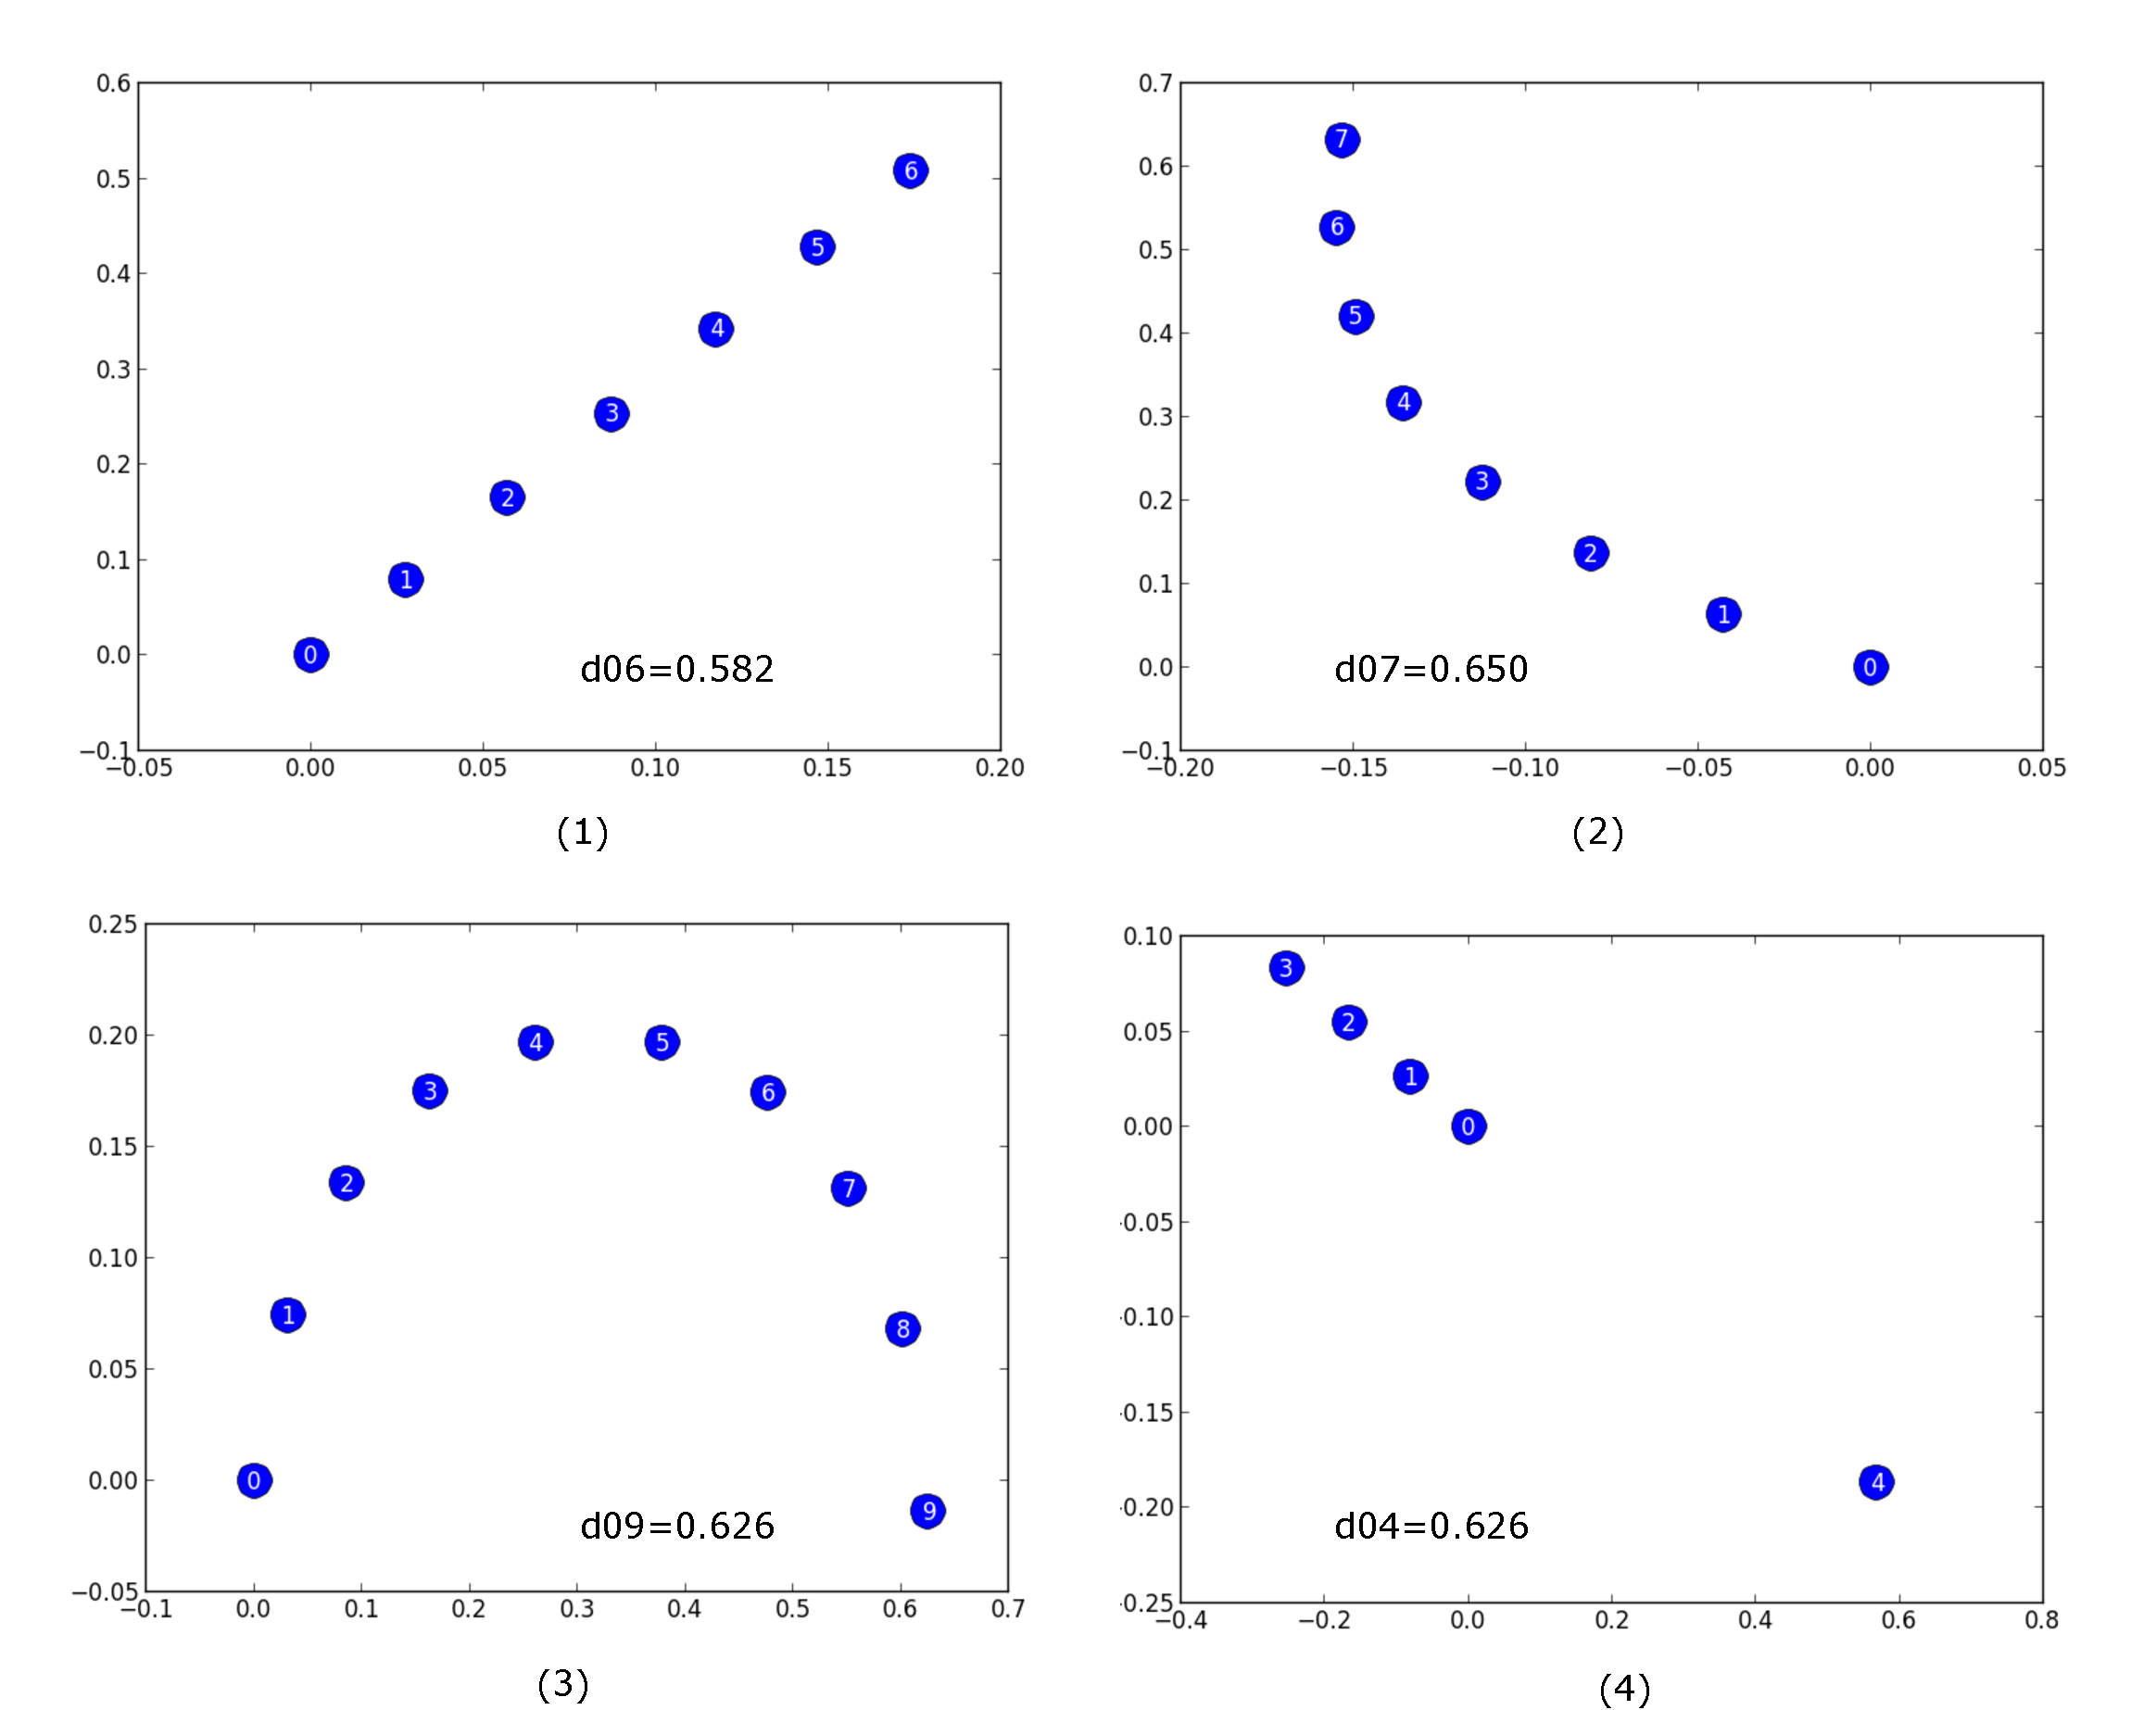
\includegraphics[height=5.0in]{Figs/demo2.pdf}
\caption{\label{demo2}The demonstration experiments of Corollary~\ref{positive path} and \ref{negative path}. Each blue ball has a white number $i$ in it, indicating node $i$'s location in its converged layout.}
\end{figure}
By Proposition~\ref{neutralization}  and Proposition~\ref{attenuation},  we further have the following two corollaries regarding positive and negative paths.
\begin{corollary}\label{positive path}
Positive Path. Given a path that consists of positive edges only, the positive relation will propagate with its strength being attenuated along the path, until it becomes a neutral relation.
\end{corollary}
Let $A_{1},A_{2},...,A_{n}$ be a positive path, such that every $(A_{1}, A_{2})$ is a positive relation. The corollary states that every $(A_{1}, A_{k})$ will be a non-negative relation, and that $(A_{1}, A_{k-1})$ will be positively stronger than $(A_{1}, A_{k})$.
\begin{corollary}\label{negative path}
Negative Path. Given a path that consists of only one negative edge, the relation between the end nodes of the negative path is non-positive in the balanced network. 
\end{corollary}
We demonstrate the transitivity and attenuation along a Positive Path in (1) (2) (3) of Figure~\ref{demo2}. (1) of Figure~\ref{demo2} shows the converged layout of a positive path consisting of $6$ strongly positive relations. In this configuration, since the sum of all $6$ distances is smaller than the relation distance of a neutral edge, all nodes stay on the same line. Clearly, $d_{06} > d_{05}>...>d_{02}$, which agrees with the attenuation property. $d_{06}$ turns to be in the range of neutral relations, which indicating the relationship between node $0$ and node $6$ becomes neutral.  

(2) (3) of Figure~\ref{demo2} show the converged layout of a positive path consisting of $7$ and $9$ strongly positive relations respectively. In such cases,  the sum of all $7$ or $9$ distances becomes larger than the relation distance of a neutral edge. As a result, the layout of nodes curves. Both $d_{07}$ and $d_{09}$ are in the range of neutral relations. Moreover, $d_{07}$ is consistently larger than $d_{09}$ in our experiments, indicating the distance between two endpoints of the positive path is non-increasing w.r.t. the path length. The empirical results of (2)(3) show the non-negativeness of the relationship between the endpoints of a positive path.

(4) of Figure~\ref{demo2} is the converged layout of a negative path, in which $(3,4)$ is the only negative edge. Similar to positive path, it has a non-positive relationship between its two endpoints.
\begin{figure}[th]
\centering
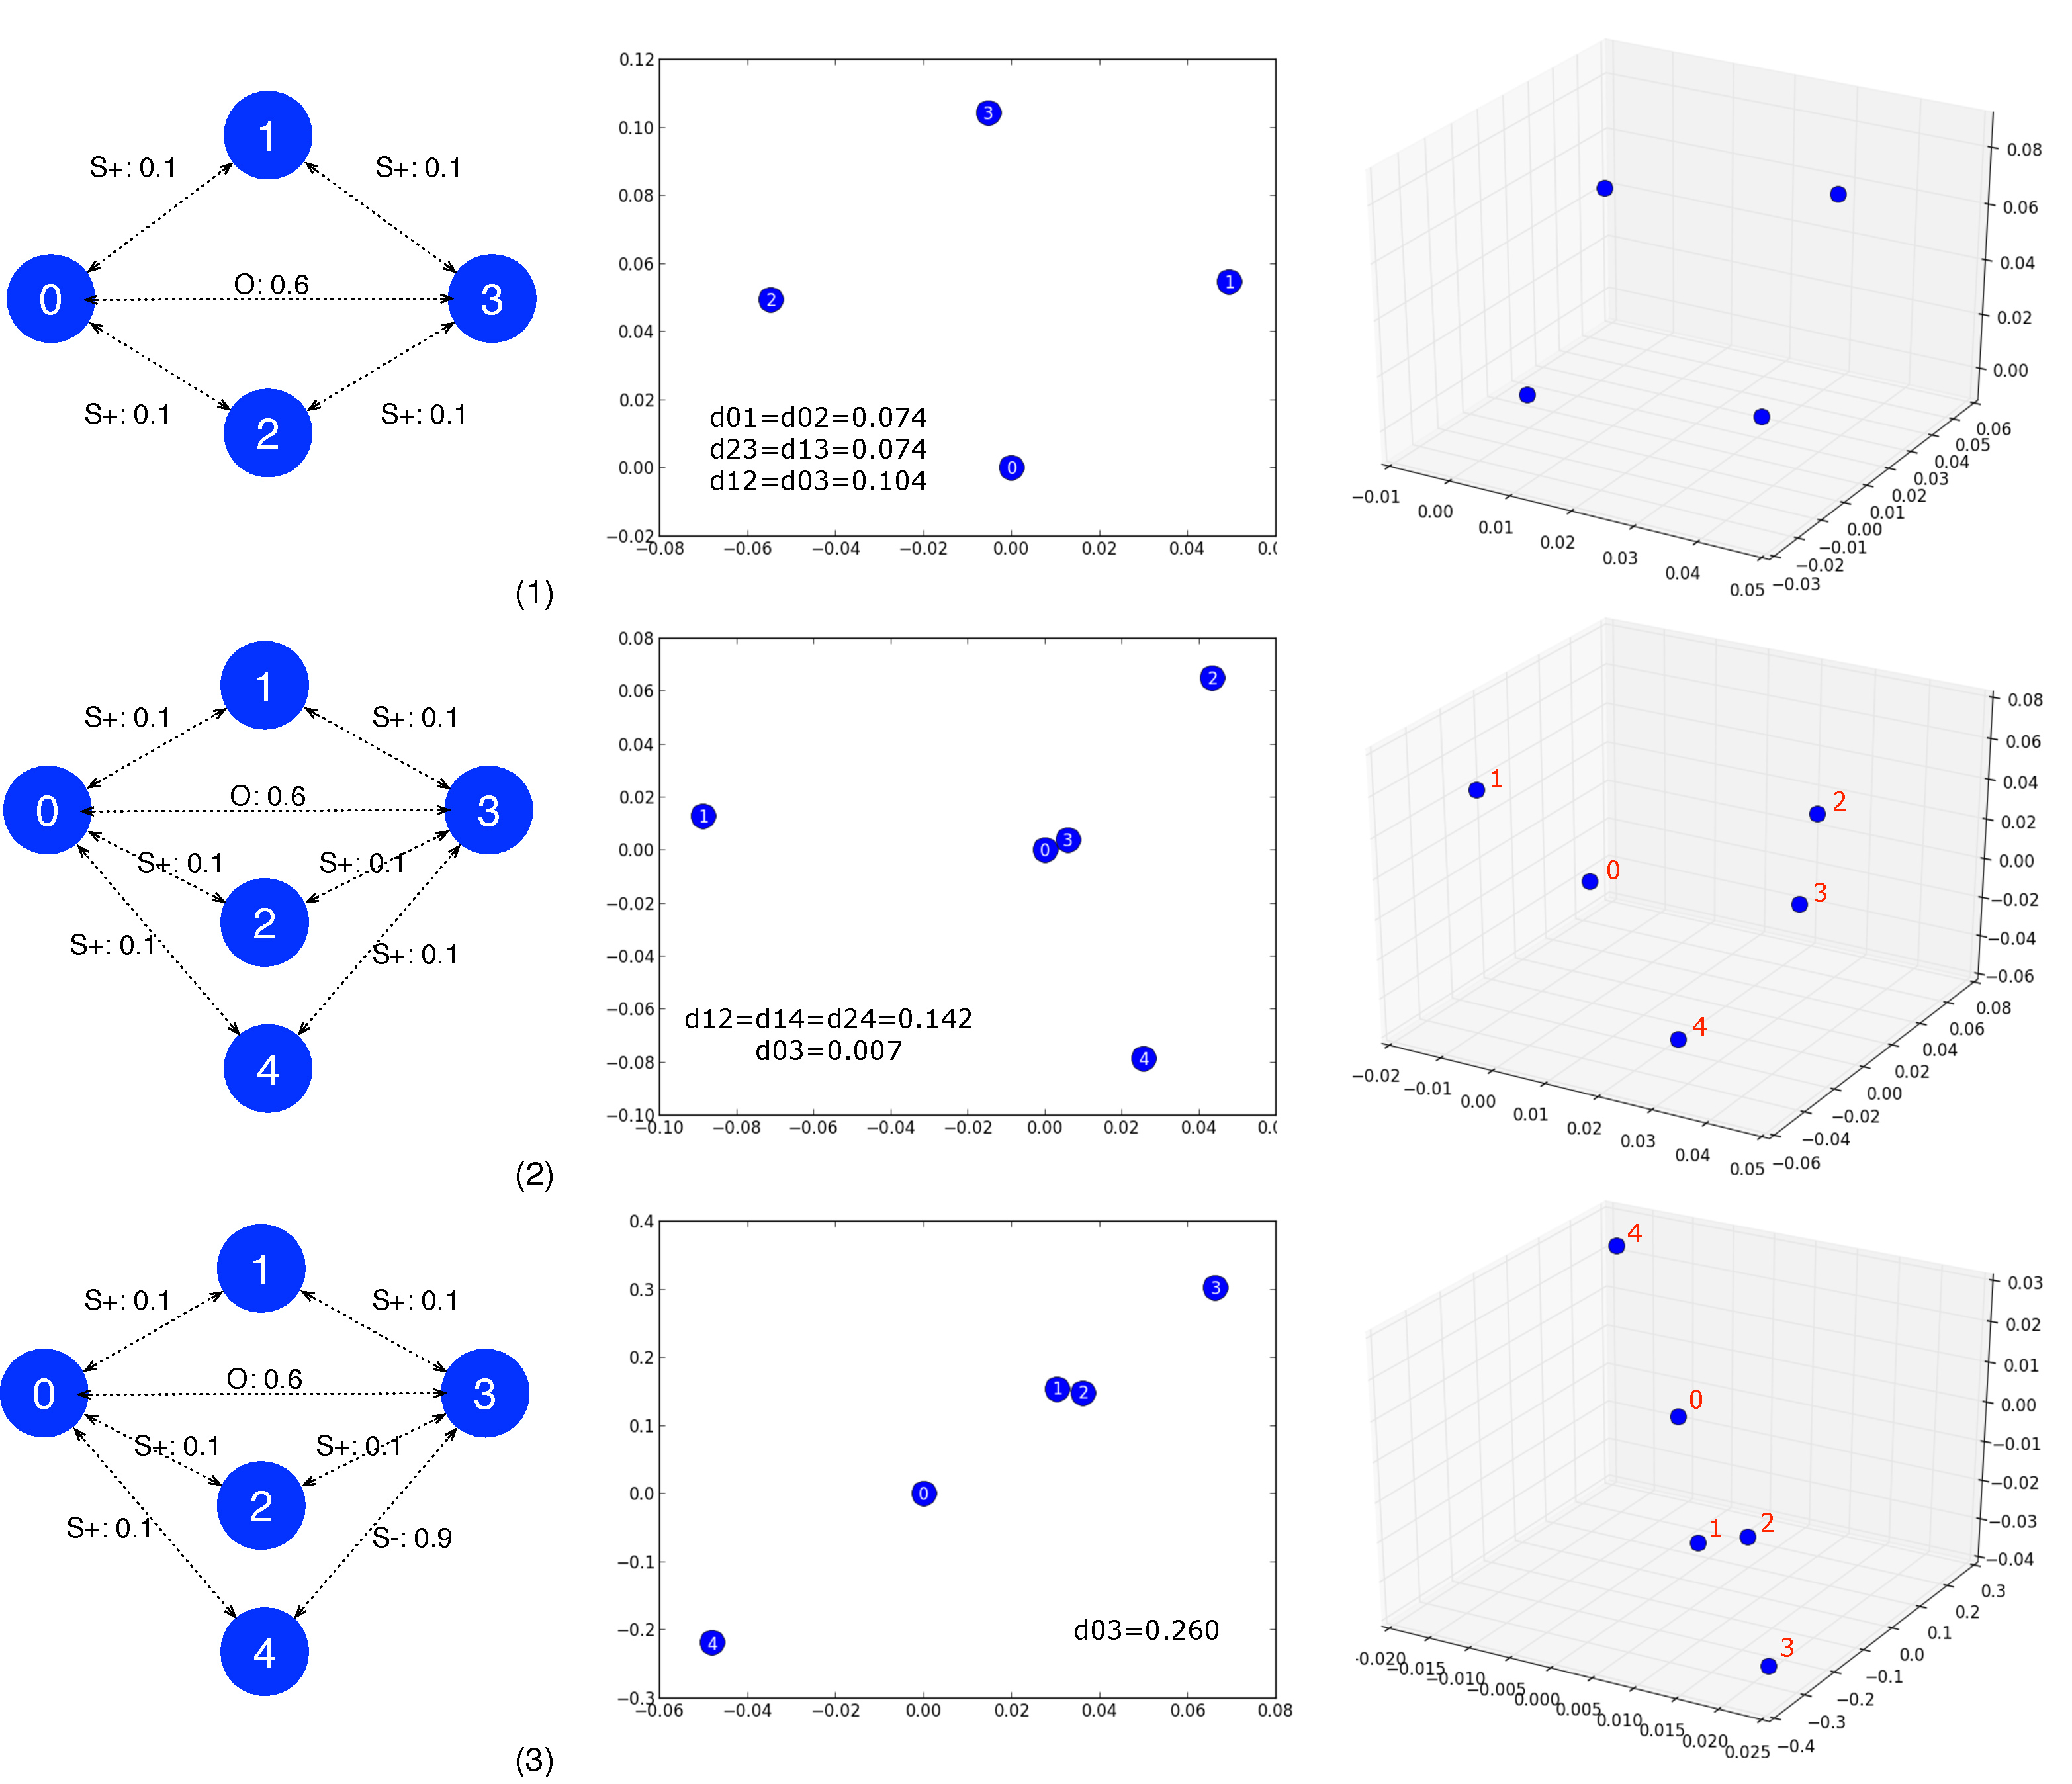
\includegraphics[height=5.0in]{Figs/demo3.pdf}
\caption{\label{demo3}The demonstration experiments of Proposition of Aggregation. Each blue ball has a white number $i$ in it, indicating node $i$. The initial state of each triad is shown in figures on the left, the corresponding converged layouts in 2-D space is shown in the middle, and the corresponding converged layouts in 3-D space is shown on the right.}
\end{figure}
\begin{proposition}\label{aggregation}
Aggregation Property. Suppose there are multiple positive and negative paths between two nodes, then adding one more positive path between them will make their relation more positive while adding one more negative path will make the relation more negative.
\end{proposition}
Aggregation property is a generalization of ``people with more common friends are more likely to become friends". It says if two people A,B have more (direct or indirect) friends in common, then they are more likely to be friends, or less likely to be enemies. On the other hand, if they have more conflicting people in common, who are (direct or indirect) friends of A and (direct or indirect) enemies of B, then they are more likely to be enemies, or less likely to be friends.  

To illustrate the Property of Aggregation, we run $3$ different tests. In the first experiment shown in (1) of Figure~\ref{demo3}, edges $(0,1),\,(0,2),\,(1,3),\,(2,3)$ are given as strongly positive initially.  The converged layout forms a square, and $d_{03}=\sqrt{2}{d_{01}}$. Obviously, $d_{03}$ is in the range of positive relations. Moreover, $d_{03}$ is smaller than $d_{02}$ in (1) of Figure~\ref{demo1}, which indicates adding a common friend between two people will grant a better chance to them to become friends. In the second experiment shown in (2) of Figure~\ref{demo3}, we add another positive path ${0,4,2}$. The converged layout is still symmetric, but the distance between node $0$ and node $3$ becomes very close, which agrees with the concept of aggregation. In the third experiment shown in (3) of Figure~\ref{demo3}, we add a negative path instead. In the converged layout, the distance between node $0$ and node $3$ becomes larger than $d_{02}$ in (1) of Figure~\ref{demo1}, which indicating adding a conflicted common neighbor between two people will deteriorate their relationship.

When the number of nodes is more than $3$, a two-dimensional drawing is not necessarily able to express the layout of minimum relation cost. For example, in (2) of Figure~\ref{demo3}, $d_{03}$ would be larger if drawing in a 3-D space. Due to the limit of dimensionality, node $0$ and node $3$ are forced to squeeze together. In studying the effects of dimensionality, we repeat the same aggregation demonstrations in 3-D space. In (1) of Figure~\ref{demo3}, the layout still forms a square. In (2) of Figure~\ref{demo3}, the layout forms a  triangular bipyramid, and the distance between node $0$ and node $3$ becomes reasonably small, but is still smaller than it is in (1) of Figure~\ref{demo3}. In (3) of Figure~\ref{demo3}, the distance between node $0$ and node $3$ is slightly larger than it is in (1) of Figure~\ref{demo3}, showing a more reasonably deterioration of relationship by adding a negative path.

{\bf Proof. } We present the general idea of the proof. See appendix for the full proof. 
Initially, strongly positive relations $(A, B)$, $(B, D)$ are given. By Proposition~\ref{closure}, the length of $(A,D)$ will be approximately $\psi(A,B)+\psi(B,D)$ in the balanced network.

Suppose one more positive paths is added between $A$ and $D$. For example, strong positive edges $(A,C)$ and $(C,D)$ are added. Neutral edge $(B,C)$ needs to stretch out to reach their initial length $b_{w+}$. But if edge $(B,C)$ stretches more, edge $(A,D)$ has to stretch less in space. In the balanced network $\cal G$, $A,B,C,D$ will form a quadrilateral in the Euclidean space. Hence, the length of $(A,D)$ will be smaller than $\psi(A,B)+\psi(B,D)$.

Moreover, with more neutral edges like $(B,C)$ on the multi-plane that is vertical to $(A,D)$, the network structure will be balanced at a point where $(A,D)$ is less stretched, so that the total relation cost is minimized. 

On the other hand, if adding one more negative path between $A$ and $D$, then equivalently a non-positive relation will be added between them according to corollary~\ref{negative path}. If it is a negative relation, $(A,D)$ will be directly stretched out, because negative relation is longer than neutral relation in metric space. $\Box$